%%%%%%%%%%%%%%%%%%%%%%%%%%%%%%%%%%%%%%%%%%%%%%%%%%%%
% ITU Ph.D. Proposal Template
% Created by Farabi Ahmed TARHAN
% @2017 06 14
%%%%%%%%%%%%%%%%%%%%%%%%%%%%%%%%%%%%%%%%%%%%%%%%%%%%

\documentclass{ituphdreport}


\thesistitle{Multi Agent Planning Under uncertainty Using Deep Q Networks}
\writer{Farabi Ahmed}{TARHAN}
\studentid{511142108}
\department{Department of Aeronautical Engineering}
\programme{Aeronautical Engineering Programme}
\ddate{2nd REPORT JUNE 2018}
\tezyoneticisi{Assist. Prof. Dr. N. Kemal Üre}{Istanbul Technical University}
\juriBir{Prof. Dr. Gökhan İnalhan}{Istanbul Technical University}
\juriIki{Assist. Prof. Dr. Yıldıray Yıldız}{Bilkent University}

\begin{document}


\section{INTRODUCTION}
% Revised
In this thesis progress report, the studies conducted at the second 6 month period of this study will be presented. As mentioned in the time plan of the thesis, it is aimed to develop a general framework that provides a basis for solving multiagent problems with deep q networks. In this context, a custom deep network framework and some benchmark problems designed and various q learning algorithms were tested over these benchmark problems. The outline of this progress report is as follows. In this section, an introduction is given and the scope of the thesis was reminded again. A time plan given in the approved proposal of the thesis was reintroduced in the 2nd Section. In Section 3, contribution of the studies conducted during the last six months within the whole thesis study is evaluated. The studies conducted during the last six months in accordance with the time plan are listed and their results are given in 4th Section. In Section 5, the studies included in time plan but not conducted are listed. In Section 6, the updated methodologies and their reasons are given. The next section explains the studies that is planned to be done for the next six months. In the last section, publications about the thesis is mentioned.

The proliferation of Unmanned Aerial Vehicles (UAVs) in the military and civil applications to substitute humans in dangerous or risky missions made UAVs very active research topic in many engineering fields. Control practices for a single vehicle or an agent had a major progress in executing advanced techniques such as adaptive control, intelligent control and robust control during the development of control theory. In the last decades, the idea of utilizing interconnected multiagent systems has gained more popularity in the continuation of the former developments, since lots of benefits can be obtained when complex solo systems are replaced by their heterogeneous and multiple counterparts \cite{rencao11}. Multiagent systems can be defined as a coordinated network of problem-solving agents, which cooperate to find answers to given problems that are otherwise impossible to accomplish or highly time-consuming jobs. In general, the required capabilities of collaborative scenarios are beyond the capabilities of a single agent \cite{glavic06}.

The most prominent reasons of why multiagent systems are advantageous when compared with solo systems can be given in terms of collaboration, robustness, and quickness in addition to scalability, flexibility and adaptivity \cite{clement04}. Since each member of a multiagent system executes small part of a complex problem, those given reasons occur inherently. Especially surveillance-like missions exploit multiple robots simultaneously since a team of robots obviously has a big return due to the geographic distribution over using just a single robot \cite{stone00}. While a single robot can execute the mission from just a single observation point, multiagent systems can perform the mission from lots of strategic points that are spread over a large area.

Due to its promising benefits, multiagent planning problems are becoming prevalent in engineering as an emerging sub-field of Artificial Intelligence (AI). Since the applications range across control of robotic missions, computer games, mobile technologies, manufacturing processes and resource allocation, it is also a widely acknowledged interdisciplinary engineering problem that draws the attention of researchers from distinct fields including computer science \cite{stone00}, aerospace engineering \cite{tomlin98}, operations research \cite{swaminathan98}, and electrical engineering \cite{glavic06}.

In this Ph.D. thesis, it is aimed to develop a highly scalable multiagent planning framework with the support of both centralized and decentralized setting for heterogeneous teams by using Deep-Q-Networks (DQN) technique to reduce dependency on the domain knowledge of the large-scale problems. Recent studies on machine learning and, in particular, on deep learning have demonstrated very promising successes in solving problems with complex and high-dimensional spaces \cite{silver2016mastering} \cite{zhang2016learning}\cite{mnih-dqn-2015}.

Centralized solutions, that require all the agents to communicate each other, will be developed using Multiagent Markov Decision Processes (MMDPs) as described in subsection \ref{sec:mmdp}. MMDPs are an extended version of standard MDP models to formulate multiagent decision-making problems. Most of the large-scale problems suffer from curse-of-dimensionality. Having high dimensional spaces such as multiagent planning problems impedes the convergence rate significantly. Centralized formulations also have large planning spaces since joint spaces of each agent is considered, hence these multiagent systems suffer from being exponential in the size of planning space as the number of agents increases \cite{redding2011approximate}. Therefore classical Dynamic Programming (DP) methods are not practical for such problems since they do not scale well. In order to reduce the computational complexity of the problem, approximate dynamic programming methods are developed to obtain at least near-optimal results. However, many of these algorithms depend on domain knowledge and extensive tuning. Recent advances in applying deep structures to multiagent systems show encouraging results \cite{hausknecht2015deep}\cite{tampuu2017multiagent}. By utilizing deep networks, the problems with large spaces can be solved by minor tuning that just comprises network topology. 

%Actor Critic
For most of the practical problems, because of the very large size of state and action spaces, computation of exact state-action values are intractable \cite{Vijaymohan2002}. When dealing with large scale problems including the ones consist continuous actions or huge discrete action spaces policy gradient based Actor-Critic algorithms are the most popular methods in reinforcement learning \cite{grondman2012survey}. Actor-Critic algorithms separate value functions and policy functions \cite{mnih2016asynchronous}. This method combines the advantages of policy gradient only methods with the conventional Deep Q-Networks and allows more robust, faster, low varianced solutions \cite{grondman2012survey}. Actor-Critic method estimates both policy and value function. There are two closely related steps in Actor-critic, actor improvement and critic evaluation. While the goal of the first part is to improve the current policy, second part only evaluates the value of current policy. 
%Actor Critic

In real-world scenarios, the agents might not communicate each other always, due to communication limits. Having a limited or sometimes accessible communication makes some of the agents to be unaware of the states of other agents and the environment. In such scenarios, some precautions must be taken into account to let the team reach a common goal. In which situations, when agents are experiencing communication troubles, each agent should take care of themselves to keep the global reward of the mission acceptable at the same time. Hence, the technique that will be utilized should allow the agents, that receive separate observations, to take actions solely based on that local information \cite{amato13}. In this thesis Decentralized Partially Observable Markov Decision Processes (Dec-POMDPs) described in subsection ~\ref{sec:decpomdp} will be utilized to formulate multiagent decision making and control problem under uncertainty. A very recent study shows that Deep Q-Networks are a very promising method to deal with large-scale problems when studying decentralized systems \cite{chen2016decentralized}.

The scope of this thesis consists of developing a framework of both MMDPs and its decentralized counterpart Dec-MDPs. In order to evaluate the performance of the framework on UAV missions, a 3D Visual Software/Hardware-In-The-Loop UAV simulator will also be developed. For the detailed evaluation of the decision-making system, 6 degree-of-freedom model of each member of the heterogeneous team, including an autonomous fixed-wing aircraft, an autonomous helicopter, and an autonomous multi-rotor, will be embedded in the simulation environment.

\section{TIME PLAN PRESENTED IN THESIS PROPOSAL}
% Revised
As proposed in the proposal report, the envisioned time plan is depicted here again with shaded area in Figure \ref{fig:timeplan}. The shaded area shows the last twelve months that passed after the presentation of proposal report, and the items that had to be done so far. According to the plan, main work packages can be summarized as preliminary works, multiagent planning, decentralized multiagent planning, preparing simulation environment and thesis completion. In the preliminary phase, some elementary algorithms, such as value iteration, trajectory-based q-iteration, and deep-q-networks, were being implemented and tested in some benchmark environments especially grid-world and its derivatives. In second work package as the main objective of this report, multiagent planning algorithms were developed and tested in the rendezvous problem an simplified version of persistent surveillance environment. Afterward, the most challenging part of the thesis, decentralized multiagent planning, will be started to be developed. Followed by that work package, the 3D simulation environment will be developed to visualize the performance of the algorithms. In the last work packages, thesis writing will be started in parallel to writing journal drafts. As proposed in the proposal report, all of the thesis is still expected to be completed in 24 months.


\begin{figure}[h]
	\begin{center}
		\resizebox{6.3in}{!}{\includegraphics*{TimePlan3}}
	\end{center}
	\caption{Time plan presented in thesis proposal.
		\label{fig:timeplan}}
\end{figure}

%\input timeplan.tex


\section{CONTRIBUTION OF THE STUDIES CONDUCTED DURING THE LAST SIX  MONTHS WITHIN THE WHOLE THESIS STUDY}
% Revised
In the last six months of the study, another type of decision making method called as Actor-Critic is integrated to previously developed deep reinforcement learning library. This new method is applied to well known decision making problems in accordance with the goals of this thesis including grid-world and rendezvous problems that were developed in the first phase of this study. Two different sets of Actor Critic methods are focused such as tabular based and deep neural network backed function approximation methods and their results were obtained. Besides these substantial works in accordance to multiagent planning and decision making, some other considerable developments are achieved. In order to reach higher convergence rate in iterative simulations in small amount of time, grid search algorithm is developed and integrated to the framework. Besides these software based improvements an machine learning focused computer with hybrid CPU and GPU is investigated and established to the machine learning laboratory. Since these conducted improvements will serve much to the convergence rate of the simulations for the whole thesis study, they were really important to be included in the framework to obtain such a general framework for multiagent decision making settings. 

\section{EXPLANATION OF THE STUDIES CONDUCTED DURING THE LAST SIX  MONTHS IN ACCORDANCE WITH THE TIME PLAN AND THEIR RESULTS} \label{sec:conductedstudies}
% Revised
This section gives technical background on the methods that are used in planning multiagent systems for this term. State-action tabular and deep neural network backed function approximation based Actor Critic method along with the grid search implementation and hybrid CPU/GPU based computer setup for simulations are explained. These tools will serve as a substantial part for the systems that are going to be developed throughout the thesis.

\subsection{Actor-Critic Reinforcement Learning} \label{sec:actorcriticrl}
Actor-critic methods originated in the Artificial Intelligence literature in the subsection of Reinforcement Learning. For most of the practical problems, because of the very large size of state and action spaces, computation of exact state-action values are intractable \cite{Vijaymohan2002}. When dealing with large scale problems including the ones consist continuous actions or huge discrete action spaces policy gradient based Actor-Critic algorithms are the most popular methods in reinforcement learning \cite{grondman2012survey}. Actor-Critic algorithms separate value functions and policy functions \cite{mnih2016asynchronous}. This method combines the advantages of policy gradient only methods with the conventional Deep Q-Networks and allows more robust, faster, low varianced solutions \cite{grondman2012survey}. Actor-Critic method estimates both policy and value function. There are two closely related steps in Actor-critic, actor improvement and critic evaluation. While the goal of the first part is to improve the current policy, second part only evaluates the value of current policy. 

As it can be seen in Figure \ref{fig:actorcritic} decision making structure includes an actor and a critic. This method combines value based and policy based methods. The actor consists some tunable parameters and at each time step, it takes a state as input and delivers an action as known as decision corresponding to its parameters. In the other side, Critic always seeks the state and rewards to evaluate and tune the policy generated by the actor \cite{Vijaymohan2002}. The value network critic evaluates the actor network and generates an error signal that guides how actor network should be modified \cite{lillicrap2015continuous}. By this way actor can always improves its current policy to achieve better decision making performance by maximizing the collected rewards. The goal of this method is to maintain a parametrized actor function $\mu(s|\theta_\mu)$ that maps s to an action deterministically as critic $Q(s,a)$ learning value of state and action pairs \cite{lillicrap2015continuous}.

\begin{figure}[h]
	\begin{center}
		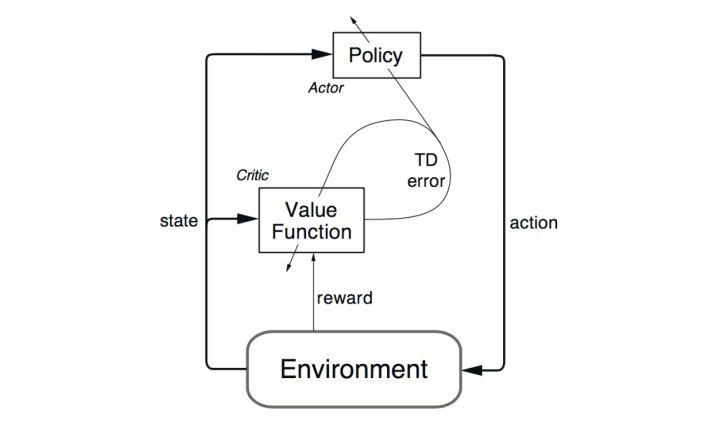
\includegraphics[width=1\textwidth]{actorcritic2}
	\end{center}
	\caption{General view of Actor-Critic Reinforcement Learning.
		\label{fig:actorcritic}}
\end{figure}

\subsubsection{Tabular Based Actor-Critic} \label{sec:actorcritictabular}
Tabular based Actor-Critic utilizes action probability matrix and state matrix to store the values of both actor and critic. Since it doesn't exploits function approximation techniques it is vulnerable to the curse of dimensionality due to is memory requirements. Hovewer, it is highly helpful to understand the basic principles of the Actor-Critic method before moving forward with the neural network based function approximators. 

\begin{figure}[h]
	\begin{center}
		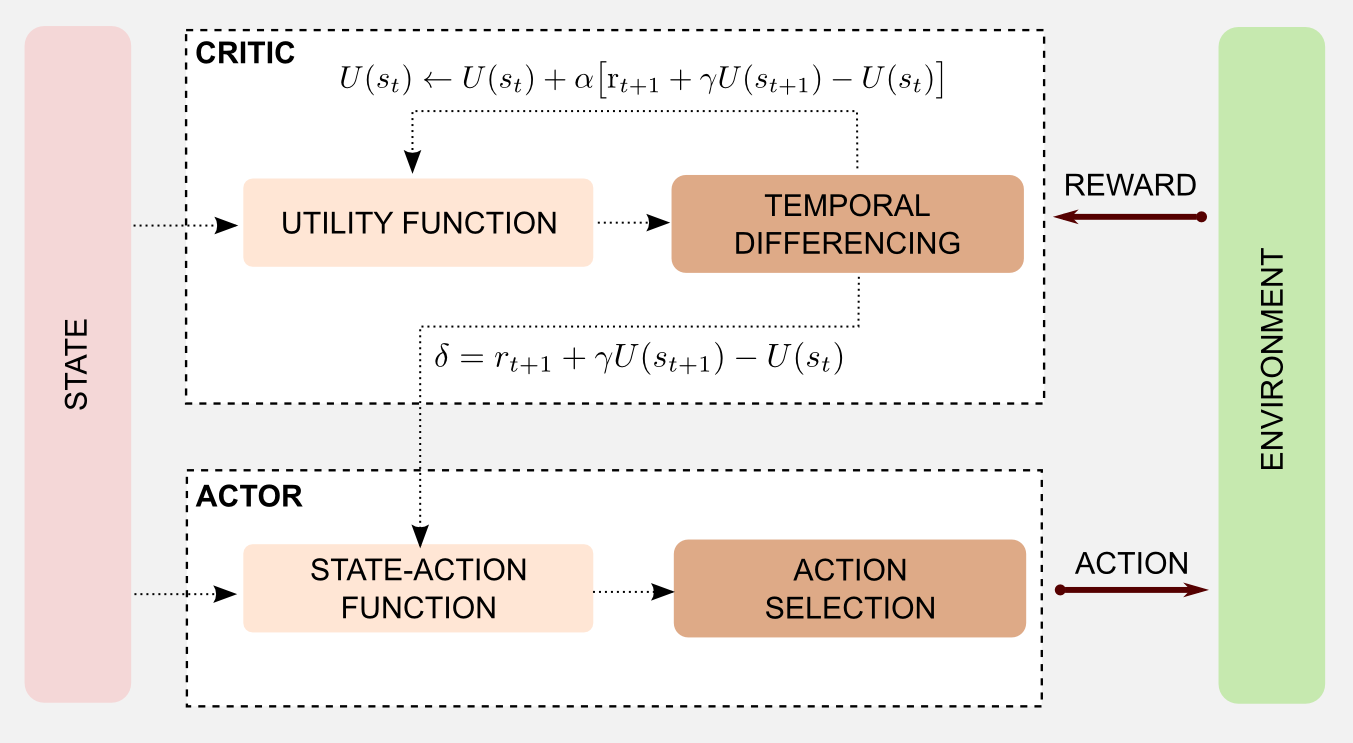
\includegraphics[width=1\textwidth]{tabularactorcritic}
	\end{center}
	\caption{Actor-Critic implementation with tabular method.
		\label{fig:actorcritic}}
\end{figure}

Figure \ref{fig:actorcritic} depicts the flow of how actor-critic works in general. The actor takes a state $s_t$ as an input and produces an action $a_t$ for the current state $s_t$ to be applied. Then, the critic observes the next state  $s_{t+1}$ and the reward $r$ from the environment. By the help of observed reward critic updates its utility function matrix for state  $s_t$. Critic also tunes the actor via $\delta$ which is the error term between recently observed reward and the current value of state. The actor selects the action according to the softmax function:

\begin{equation}
\label{eq:acsoftmax}
P \{a_t = a | s_t = s\} = \frac{e^{p(s,a)}}{\sum_{b}^{} e^{p(s,b)} }
\end{equation}

where $P{a_t|s_t}$ is the probability of selecting action $a_t$ in state $s_t$ and $p(s,a)$ is the stored value of actor function for the state-action pair. Since critic only stores state values instead of state-action values, it is called utility function. With the observed reward and next state, the utility function is updated as TD(0) as follows:

\begin{equation}
\label{eq:acutilityupdate}
U(s_{t}) \leftarrow U(s_{t}) + \alpha \big[ \text{r}_{t+1} + \gamma U(s_{t+1}) - U(s_{t}) \big]
\end{equation}

Actor is updated according the error $\delta$ and a learning rate:

\begin{equation}
\label{eq:acactorupdate}
p(s_{t}, a_{t}) \leftarrow p(s_{t}, a_{t}) + \beta \delta_{t}
\end{equation}

Where prediction error $\delta$ generated by critic is calculated as follows:

\begin{equation}
\label{eq:acdeltaerror}
\delta_{t} = r_{t+1} + \gamma U(s_{t+1}) - U(s_{t})
\end{equation}



\subsubsection{Deep Neural Network Based Actor-Critic} \label{sec:actorcriticdnn}
The most of the Reinforcement Learning and Neuro Dynamic Programming techniques are classified in either actor only or critic only methods. Since actor only methods based on policy gradient techniques, they have desirable convergence properties over critic only methods \cite{konda2000actor}. However, critic only methods are combined with the policy gradients since they exhibit high variances. As practical problems that consists large state-action spaces require tractable solutions, tabular based approaches can not be utilized due to their need to huge memory spaces. Therefore, the vast majority of the reinforcement learning methods utilize function approximators such as neural networks to represent their estimators \cite{mnih2016asynchronous}. In an actor-critic setting, the actor steers the policy of the agent which is represented by a function approximator, in the direction of the action-value gradient and the critic updates the action-value function, represented by another function approximator, using neural fitted-Q learning which is an approximate value iteration via batch learning \cite{silver2014deterministic}. In the context of reinforcement learning there are two policy methods applied including stochastic and deterministic as given in Figure \ref{fig:policydeterministicstochastic}. The stochastic policy is given by,

\begin{equation}
\label{eq:abc}
a\sim\pi_\theta(s,a)
\end{equation}

where action $a$ is sampled from a probability density function and its deterministic counterpart is given as,
\begin{equation}
\label{eq:abc}
a=\pi_\theta(s) 
\end{equation}


\begin{figure}[h]
	\begin{center}
		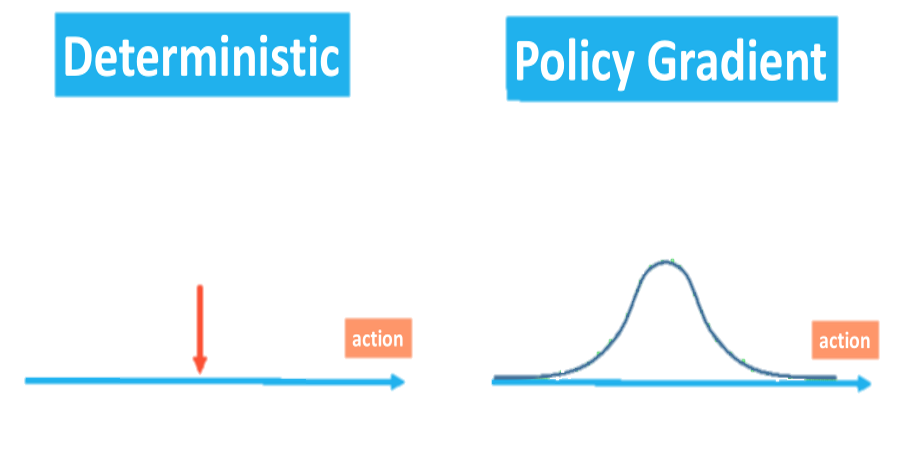
\includegraphics[width=0.6\textwidth]{policydeterministicstochastic}
	\end{center}
	\caption{Deterministic vs stochastic policies.
		\label{fig:policydeterministicstochastic}}
\end{figure}


where action $a$ is a result of direct mapping from state $s$. Each policy is parameterized by $\theta$ since they are represented by function approximators. A policy is applied to select appropriate actions for an agent that will interact with the environment to collect rewards. At each time step $t$, the agent takes an reward $r_t$ and moves to the next state $s_{t+1}$. Rewards are discounted by $\gamma$ to increase the relative importance of immediate rewards other than long-term rewards. The goal of the agent is to maximize the sum of discounted future rewards that is defined as,

\begin{equation}
\label{eq:abc}
R_t = \sum_{k=1}^{\infty}\gamma^{k-1}r_{t+k}
\end{equation}

The state-action value function is also given as,

\begin{equation}
\label{eq:abc}
Q^\pi(s,a) = \mathbb{E}_{\pi} \big[R_t|s_t = s, a_t = a\big]
\end{equation}

The objective function that is sought to be maximized is given as,

\begin{equation}
\label{eq:abc}
J(\theta) = \mathbb{E}_{\tau \sim Pr(\tau | \theta)} [R(\tau)] = \sum_{\tau} Pr(\tau | \theta) R(\tau)
\end{equation}

where $\tau$ denotes a trajectory. In order to apply optimization methods over the policy parameter $\theta$, the gradient of the objective function with respect to the policy parameter is required. 

\begin{align}
\label{eq:abc}
%\begin{split}
\nabla_\theta J(\theta)  &= \sum_{\tau} \nabla_\theta Pr(\tau | \theta) R(\tau) \\
						&= \sum_{\tau} Pr(\tau | \theta) \frac{\nabla_\theta Pr(\tau | \theta) }{Pr(\tau | \theta) } R(\tau) \\
						&= \sum_{\tau} Pr(\tau | \theta) \nabla_\theta \log Pr(\tau | \theta) R(\tau)
%\end{split}
\end{align}

If we invoke $Q^\pi(s,a)$ and expand the trajectory;

\begin{equation}
\label{eq:abc}
\nabla_\theta J(\theta) = \frac{1}{T}\sum_{t=1}^{T} Q^\pi(s,a) \nabla_{\theta} \log \pi_\theta (a_t|s_t)
\end{equation}

At this point, another parametrization $\omega$ for state-action value can be injected here since, $Q^\pi(s,a) \approx \hat{Q}(s,a;\omega)$. This introduced approximate value is the critic function approximator that will estimate the state-action value function. Gradient of policy objective function then becomes,

\begin{equation}
\label{eq:abc}
\nabla_\theta J(\theta) = \frac{1}{T}\sum_{t=1}^{T} \hat{Q}(s,a;\omega) \nabla_{\theta} \log \pi_\theta (a_t|s_t)
\end{equation}


In general, introducing such a function approximator 
$\hat{Q}(s,a;\omega)$ in place of true state-action value $Q^\pi(s,a)$ may cause a bias \cite{silver2014deterministic}. However, if $\omega$ is optimized in a way that cares these two constraints,

\begin{equation}
		\label{eq:qlineartofeatures}
		\hat{Q}(s,a;\omega) = \nabla_{\theta} \log \pi_\theta (a|s)^T\omega \\
\end{equation}
\begin{equation}
	\begin{aligned}
	\label{eq:qlinearreg}
	\underset{\omega}{{minimize }} & & J(\omega) 
	\end{aligned}
\end{equation}

 
there is no bias \cite{sutton2000policy}. Constrain \ref{eq:qlineartofeatures} says that function approximator should be linear to the features of the stochastic policy $\nabla_{\theta} \log \pi_\theta (a|s)$ and constrain \ref{eq:qlinearreg} requires that $\omega$ should be solution to linear regression problem. Objective function for the linear regression problem can be given by,

\begin{align}
	\label{eq:abc}
	J(\omega) &=  \mathbb{E}_{a \sim \pi_\theta}[(\hat{Q}(s,a;\omega) - Q^\pi(s,a))^2]
\end{align}


\iffalse
The gradient of state-action value estimation objective function is given by,

\begin{align}
	\label{eq:abc}
	\nabla_\omega J(\omega) =  \mathbb{E}_{a \sim \pi_\theta}[(\hat{Q}(s,a;\omega) - Q^\pi(s,a))^2]
\end{align}
\fi

Since our goal is to optimize both $\theta$ and $\omega$ in a way that they will cause the agent to maximize objective function, these parameters should be tuned. Gradient based optimized methods can be applied as,

\begin{align}
\label{eq:abc}
\theta_{t+1} &= \theta_t + \alpha_{\theta} \nabla_\theta J(\theta) \\
\omega_{t+1} &= \omega_t - \alpha_{\omega} \nabla_\omega J(\omega)
\end{align}

If the terms are expanded optimization steps given below can be obtained,

\begin{align}
	\label{eq:abc}
	\delta_t &= r_t + \gamma \hat{Q}(s_{t+1},a_{t+1};\omega)  - \hat{Q}(s_t,a_t;\omega) \\
	\omega_{t+1} &= \omega_t - \alpha_{\omega} \delta_t \nabla_\omega \hat{Q}(s_t,a_t;\omega) \\
	\theta_{t+1} &= \theta_t + \alpha_{\theta} \nabla_{\theta} \pi_\theta (s_t) \nabla_a \hat{Q}(s_t,a_t;\omega)|_{a=\pi_\theta (s_t)}
\end{align}

where $\delta$ denotes the temporal differencing obtained by transition to new state.

\subsection{Hybrid CPU/GPU Computation} \label{sec:hybridcomputation}
GPUs are already proved that they are the best at operations that require parallel processing such as prediction and training of neural networks \cite{rizvi2017optimized}. Therefore, large Deep Neural Networks highly utilize GPUs as both their forward and back propagation consist numerous matrix operations at each pass \cite{babaeizadeh2016ga3c}. Besides the need of GPU for training deep networks in a reinforcement learning setting, CPUs are also utilized much since any other serial operations such as interaction with environment requires powerful serial processors. Exploring different parts of the environment with different exploration policies can be done by multiple CPUs and feeds the learner faster \cite{mnih2016asynchronous}. 

Figure \ref{fig:acframeworkoverview} shows the integration of multiple CPU and GPU to make a hybrid system. The recently developed DNN based Actor-Critic method is designed in a way that uses both GPU and multiple CPU. Different instances of Actor-Critic agent are supposed to be started on CPUs. Both function approximators of actor and critic utilizes GPU since they require parallel processing power due to backward and forward operations.

\begin{figure}[h]
	\begin{center}
		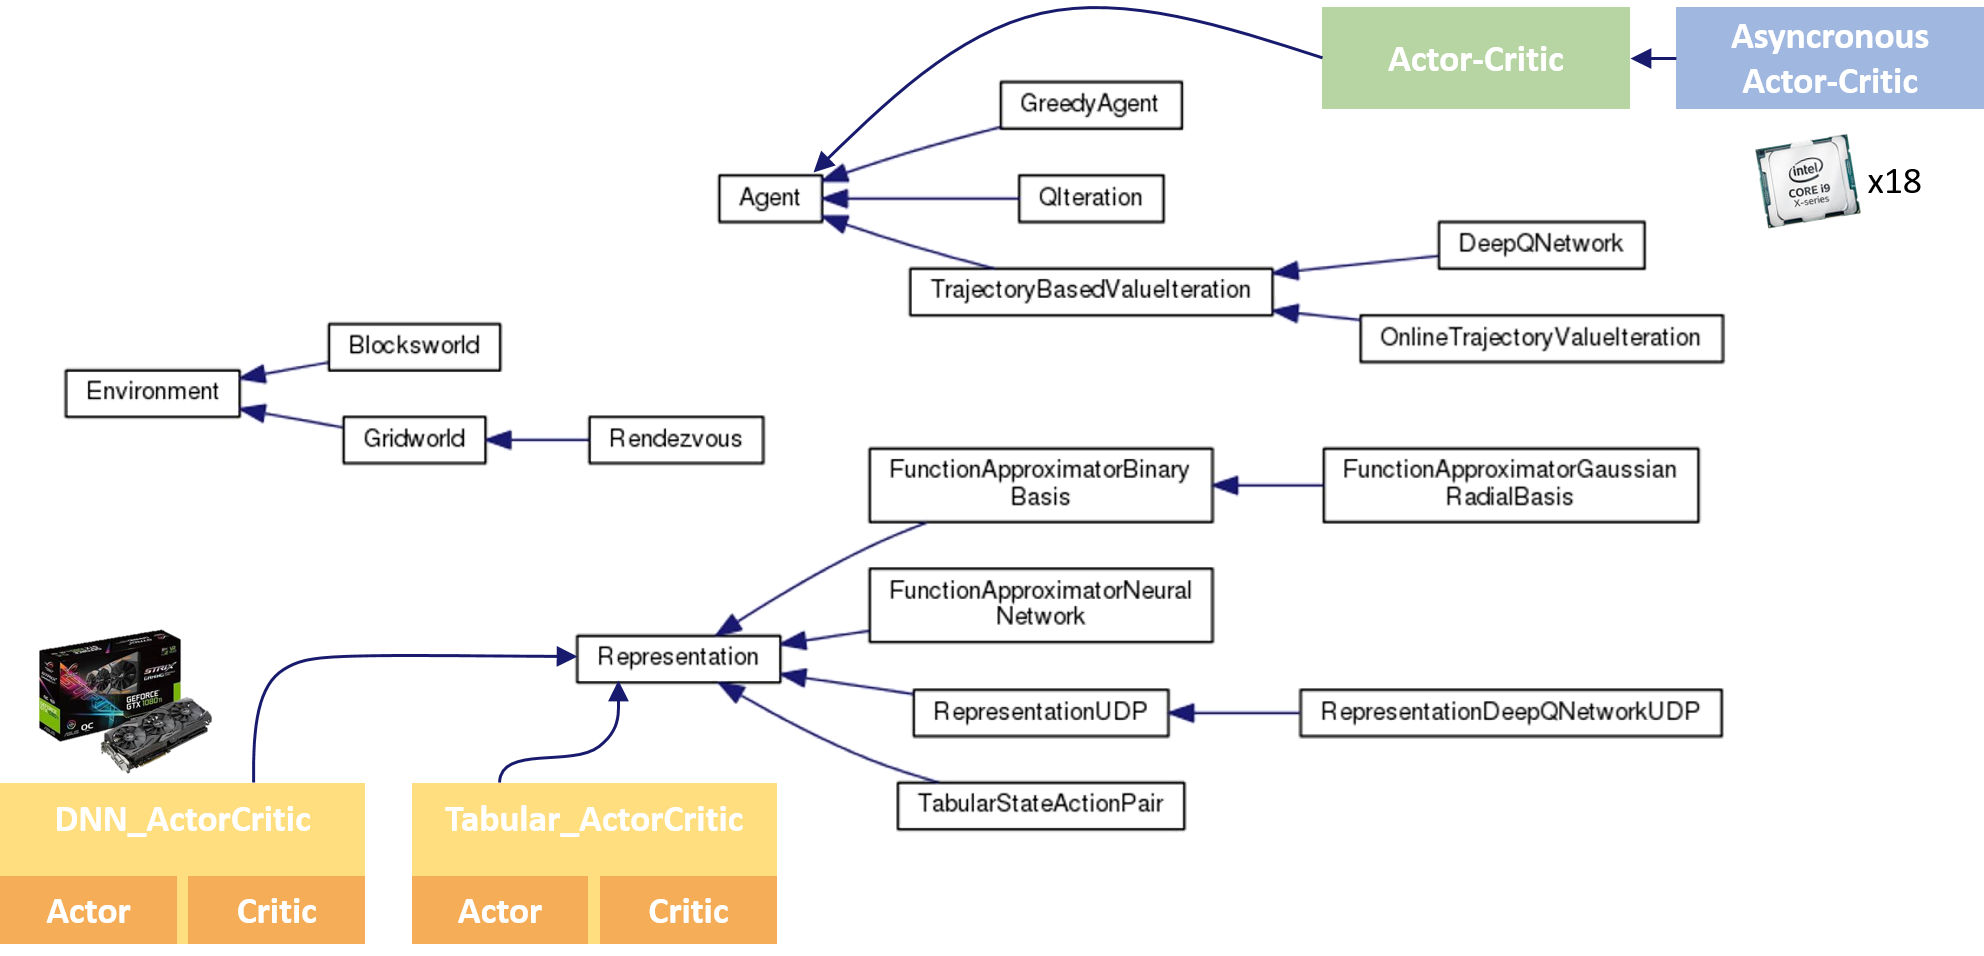
\includegraphics[width=1\textwidth]{acframeworkoverview}
	\end{center}
	\caption{Actor-Critic integration to framework utilizing hybrid CPU/GPU.
		\label{fig:acframeworkoverview}}
\end{figure}


\subsubsection{GPU/CPU Utilization} \label{sec:gputilizaiton}
GPU utilization is an monitoring parameter that shows how efficiently the learning agent utilizing the parallel processing power of the GPU. Table \ref{fig:gpuutilization} shows GPU utilization and computation times of different learning settings. Two different system settings are used. First system only employs a Intel Core i7 cpu and no GPU that supports CUDA/CuDNN while the second system employs a Intel Quad 8400 CPU and a GTX1050TI GPU that supports CUDA/CuDNN. 

First row of the table shows that using a GPU with \%80 utilization highly improves the computational time. Mnist is a dataset that consists collection of handwritten numbers. Since it is a good benchmark dataset that is highly appropriate for parallel computation it easily increased GPU utilization to higher value. Second row revealed that a reinforcement learning agent can not utilize the GPU as a conventional deep learning operation as in first row by utilizing the GPU at most \%30. Different settings of reinforcement learning agents are given in 3rd and 4th rows of the table. Besides conventional deep neural network operations, there are lots of serial computational power requirement in a reinforcement learning setting, as the interaction of environment requires CPU power instead of GPU. In order to utilize GPU computational power more, experience replay buffer should be filled faster by utilizing multiple CPU system. Asynchronous exploration agents should be employed to provide more experience tuples. 

\begin{figure}[h]
	\begin{center}
		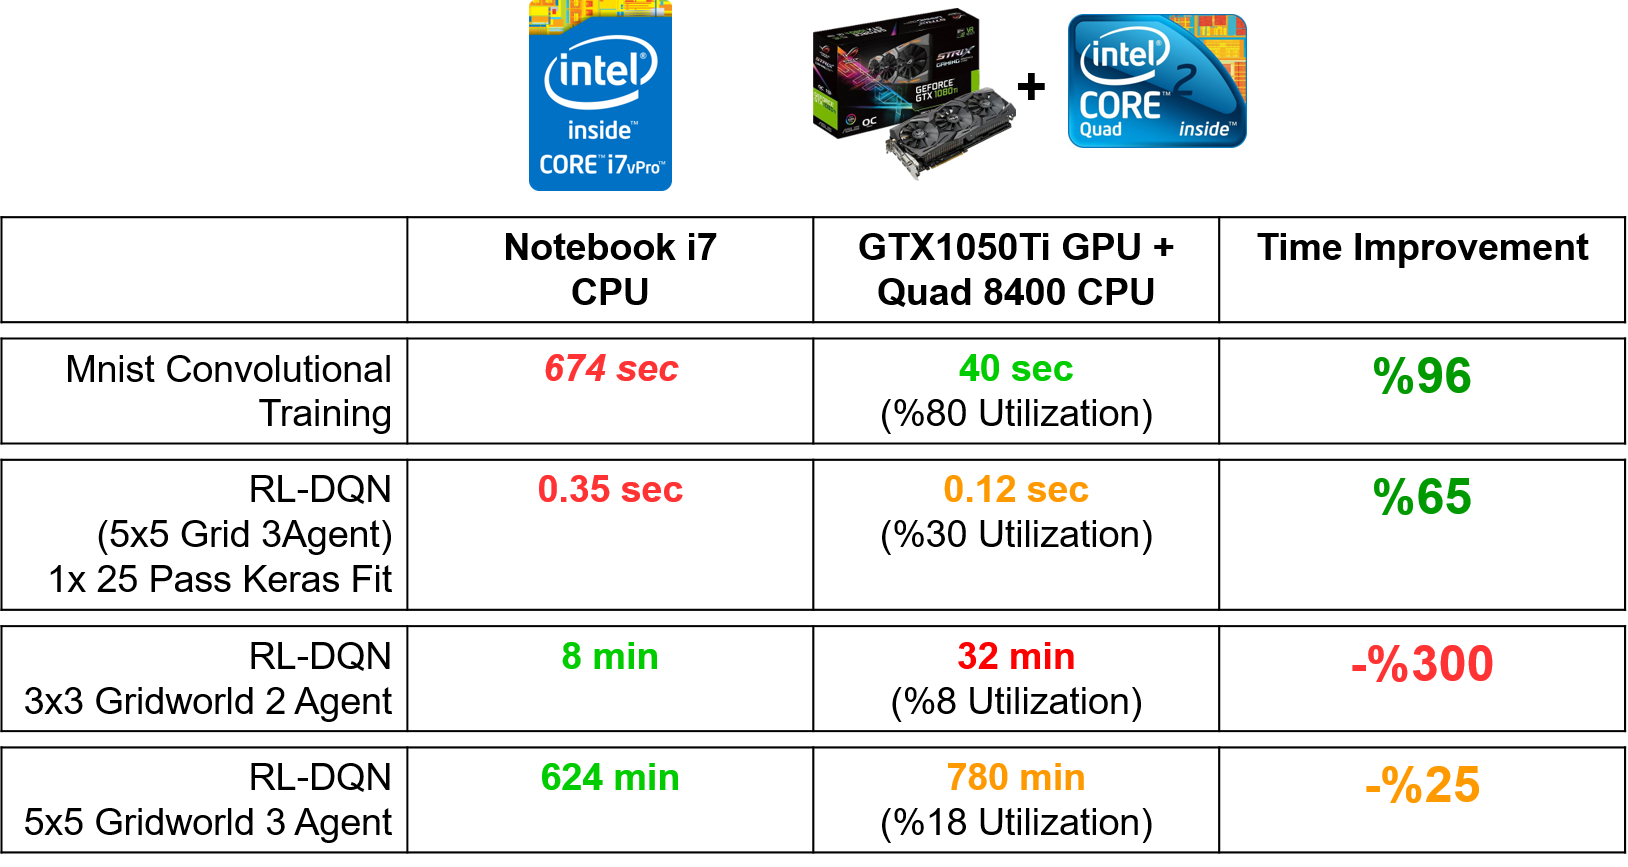
\includegraphics[width=1.0\textwidth]{gpuutilization}
	\end{center}
	\caption{GPU utilization of a hybrid system.
		\label{fig:gpuutilization}}
\end{figure}


Figure \ref{fig:cpupower} shows the utilization of different CPUs according to type of operating system. In order to evaluate the performance of CPU, 80k Bellman updates are employed. It can be clearly seen that Ubuntu OS performed faster than Windows OS in both CPU settings. Besides the operating system, Intel i9 outperformed the Intel i7 in same operation frequency of 2.6Mhz.
\begin{figure}[h]
	\begin{center}
		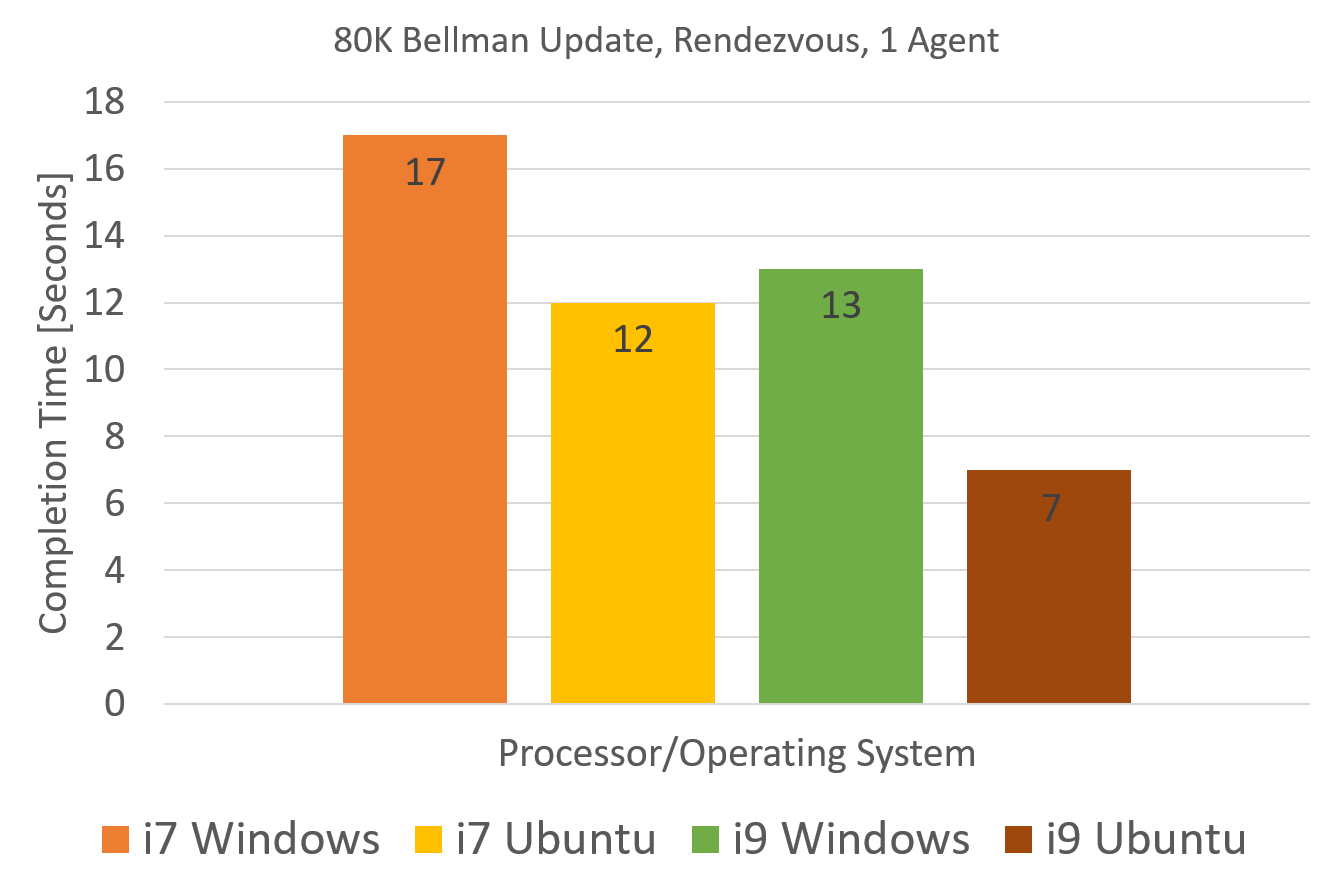
\includegraphics[width=0.6\textwidth]{cpupower}
	\end{center}
	\caption{CPU computational power comparison with different CPUs and operating systems.
		\label{fig:cpupower}}
\end{figure}


\iffalse
\subsubsection{Multi Processing vs Multi Threading} \label{sec:processvsthread}
Lorem ipsum dolor sit amet, consectetur adipiscing elit, sed do eiusmod tempor incididunt ut labore et dolore magna aliqua. Ut enim ad minim veniam, quis nostrud exercitation ullamco laboris nisi ut aliquip ex ea commodo consequat. Duis aute irure dolor in reprehenderit in voluptate velit esse cillum dolore eu fugiat nulla pariatur. Excepteur sint occaecat cupidatat non proident, sunt in culpa qui officia deserunt mollit anim id est laborum.
\fi

\subsubsection{Building Hybrid System} \label{sec:buildinghybrid}
Table \ref{table:hybridsystem} shows the main components that are assembled to build a hybrid deep reinforcement learning computer. As it is mentioned in Section \ref{sec:gputilizaiton} in order to utilize GPU's parallel computation power at most, experience replay buffer should be updated faster. Thereof, Intel Core i9 with 36 logical cores is selected as the main CPU to run asynchronous exploring agents. Besides CPU's serial computational power, operations on the DQN requires parallel computation power as GPU does. There are two main operations on deep networks including forward and backward propagation. Forward propagation is triggered when network is required to predict while backward propagation is required to train the network. In order to run both training and prediction simultaneously, two GPU's are integrated to our Hybrid system. 
 
\begin{table}
	\centering
	\begin{tabular}{ll} 
		\hline
		CPU      & Intel Core i9-7980XE @ 2.60GHz; Cores: 36 logical / 18 physical  \\
		\hline
		GPU1      & Nvidia GeForce GTX 1080 TI PCIE: 3, GDDR5X 11GB, 352-bit, Core 3584            \\ 
		\hline
		GPU2      & Nvidia GeForce GTX 1050 TI PCIE: 3, GDDR5 4GB, 128-bit, Core 768            \\ 		
		\hline
		RAM      & 2x Kingston 16GB Hyperx 3000MHz DDR4 CL17 Ram HX430C15PB3/16  \\
		\hline			
		Software & Python 3.5; CUDA 7.5 (CUDNN v5.1); TensorFlow r1.01          \\ 
		\hline		
	\end{tabular}
	\caption{Hybrid CPU/GPU configuration.
	\label{table:hybridsystem}}
\end{table}



\subsection{Grid Search Implementation} \label{sec:gridsearchimplementation}
Grid search is a method to find the optimum model hyperparameters such as hidden units, activation functions, experience buffer sizes, batch sizes, exploration parameters, etc. Neural networks are notoriously difficult to optimize since there are a lot of hyperparameters. Optimizing such hyperparameters is one of the biggest part of deep learning. Each individual should be simulated with a certain configuration and some cost function should be defined and recorded for evaluation at the end. In order to support the grid search capability to tune the hyperparameters, upper level supervisor like executable is designed as shown in Figure \ref{fig:gridsearchimplementation}. Each configuration can be added to a file that will be given as an command line configuration parameter to the grid search executable. Since the results of the grid search feature will be highly utilized during this study, it will serve as an infrastructure for the reinforcement learning framework. 

\begin{figure}[h]
	\begin{center}
		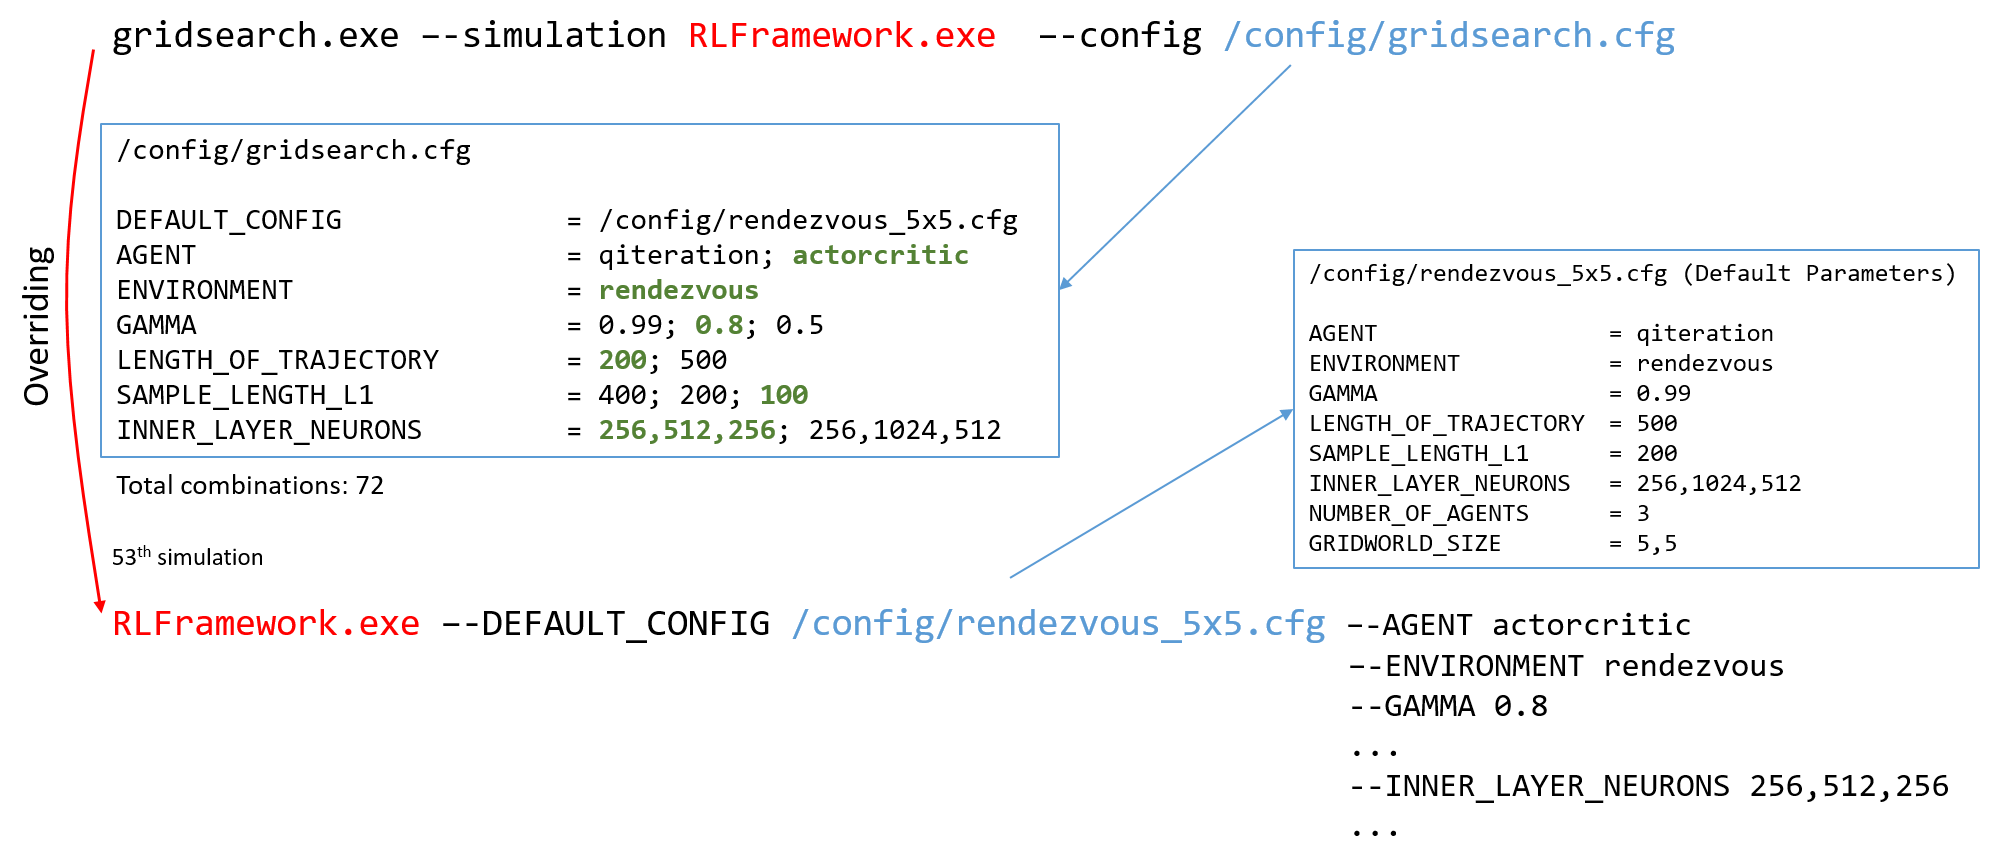
\includegraphics[width=1\textwidth]{gridsearchimplementation}
	\end{center}
	\caption{Overview of grid search implementation on C++.
		\label{fig:gridsearchimplementation}}
\end{figure}


\subsection{Simulation Results} \label{sec:simulationresults}
This section mentions the simulation results that are simulated via grid search feature. Figure \ref{fig:simPrioDQN} shows conventional critic based Deep Q Network simulation results with prioritized experience replay is on. The parameters given in Table \ref{fig:simPrioDQN} shows the hyperparameters used to run the grid search. It is obvious that a comparison mechanism is needed to find the best parameter set that converges faster and maximizes the objective function. 

\begin{figure}[H]
	\begin{center}
		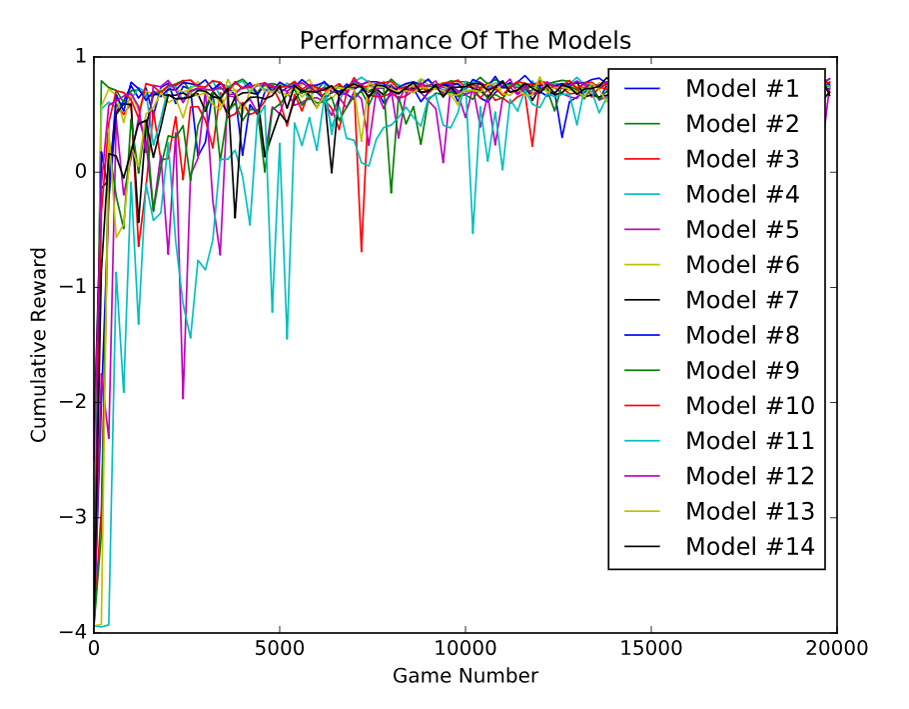
\includegraphics[width=0.6\textwidth]{simPrioDQN}
	\end{center}
	\caption{Grid search results of different models for prioritized deep q networks parameter search.
		\label{fig:simPrioDQN}}
\end{figure}

\begin{table}[]
	\begin{center}
	\begin{tabular}{lllll}
Index &	Batch Size	& Epsilon Probability	& Experience Replay	& Hidden Layers \\
\hline
1	&32	&0.2	&128	&64 \\
2	&32	&0.2	&128	&64 \\
3	&32	&0.2	&128	&32\\
4	&32	&0.2	&128	&32\\
5	&32	&0.2	&128	&16\\
6	&32	&0.2	&128	&16\\
7	&32	&0.2	&512	&64\\
8	&32	&0.2	&512	&64\\
9	&32	&0.2	&512	&32\\
10	&32	&0.2	&512	&32\\
11	&32	&0.2	&512	&16\\
12	&32	&0.2	&512	&16\\
13	&32	&0.2	&4096	&64\\
14	&32	&0.2	&4096	&64
	\end{tabular}
	\caption{Prioritized Deep Q Network Grid Search Parameters
	\label{table:priodqnsim}}
\end{center}
\end{table}

Figure \ref{fig:acgridsearch} shows the tabular based Actor-Critic algorithm with different action selection methods that are given in Table \ref{table:actabularparams} are applied. It can be clearly seen that increasing the number of samples to select action from a probability distribution make sense since it highly improves the convergence of the algorithm. Here, zero sample denotes to select the action without sampling that has highest probability. Since the simulation results for Actor-Critic algorithm with function approximators are not extensively completed yet, their results will be given in the next report.
 
\begin{figure}[H]
	\begin{center}
		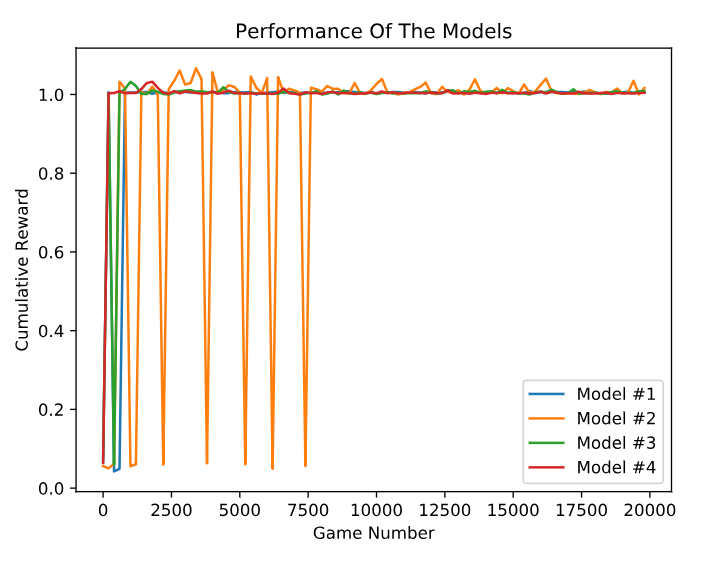
\includegraphics[width=0.6\textwidth]{acgridsearch}
	\end{center}
	\caption{Grid search results while finding optimum value for action selection of actor-critic method.
		\label{fig:acgridsearch}}
\end{figure}

\begin{table}[]
	\begin{center}
		\begin{tabular}{lllll}
			Index &	Action Selector Samples	& Elapsed Time [sec] \\
			\hline
			1	& 0		&  95 \\
			2	& 1		& 392 \\
			3	& 100	& 144 \\
			4	& 1000	& 153 
		\end{tabular}
		\caption{Tabular Actor Critic Simulation with different action selection policies
			\label{table:actabularparams}}
	\end{center}
\end{table}

\section{STUDIES DURING THE LAST SIX MONTHS INCLUDED IN TIME PLAN BUT NOT CONDUCTED AND REASONS}
% Revised
There is no study that is not conducted during the last six months. 

\section{CHANGES IN THE METHODOLOGY AND THEIR REASONS}
% Revised
There is no change in the methodology.

\section{EXPLANATION OF THE STUDIES PLANNED FOR THE NEXT SIX MONTHS}
% RevisedXXX
According to plan, in the next work package, both decentralized multiagent planning algorithms will be developed and UAV simulations will be finished on persistent surveillance environment. In order to get the most of hybrid CPU/GPU based system, an asynchronous deep decision making architecture is required \cite{stooke2018accelerated}. The proposed architecture that can be seen in Figure \ref{fig:asyncronousArchitecture} will be integrated to our custom framework. This architecture distributes serial process to CPU and parallel processes to GPU and offers higher convergence rates for multiagent decision making problems \cite{babaeizadeh2016reinforcement}. Asynchronous deep learning methods exploits multi-threading of conventional CPUs, executes many instances of agents in parallel, shares the network parameters between threads, exploits parallelism to have decorrelated data, might be an alternative to experience replay \cite{gasicdrl}.  Besides this asynchronous architecture decentralized multiagent planning methods will be started to studied and implemented to our custom framework.

\begin{figure}[H]
	\begin{center}
		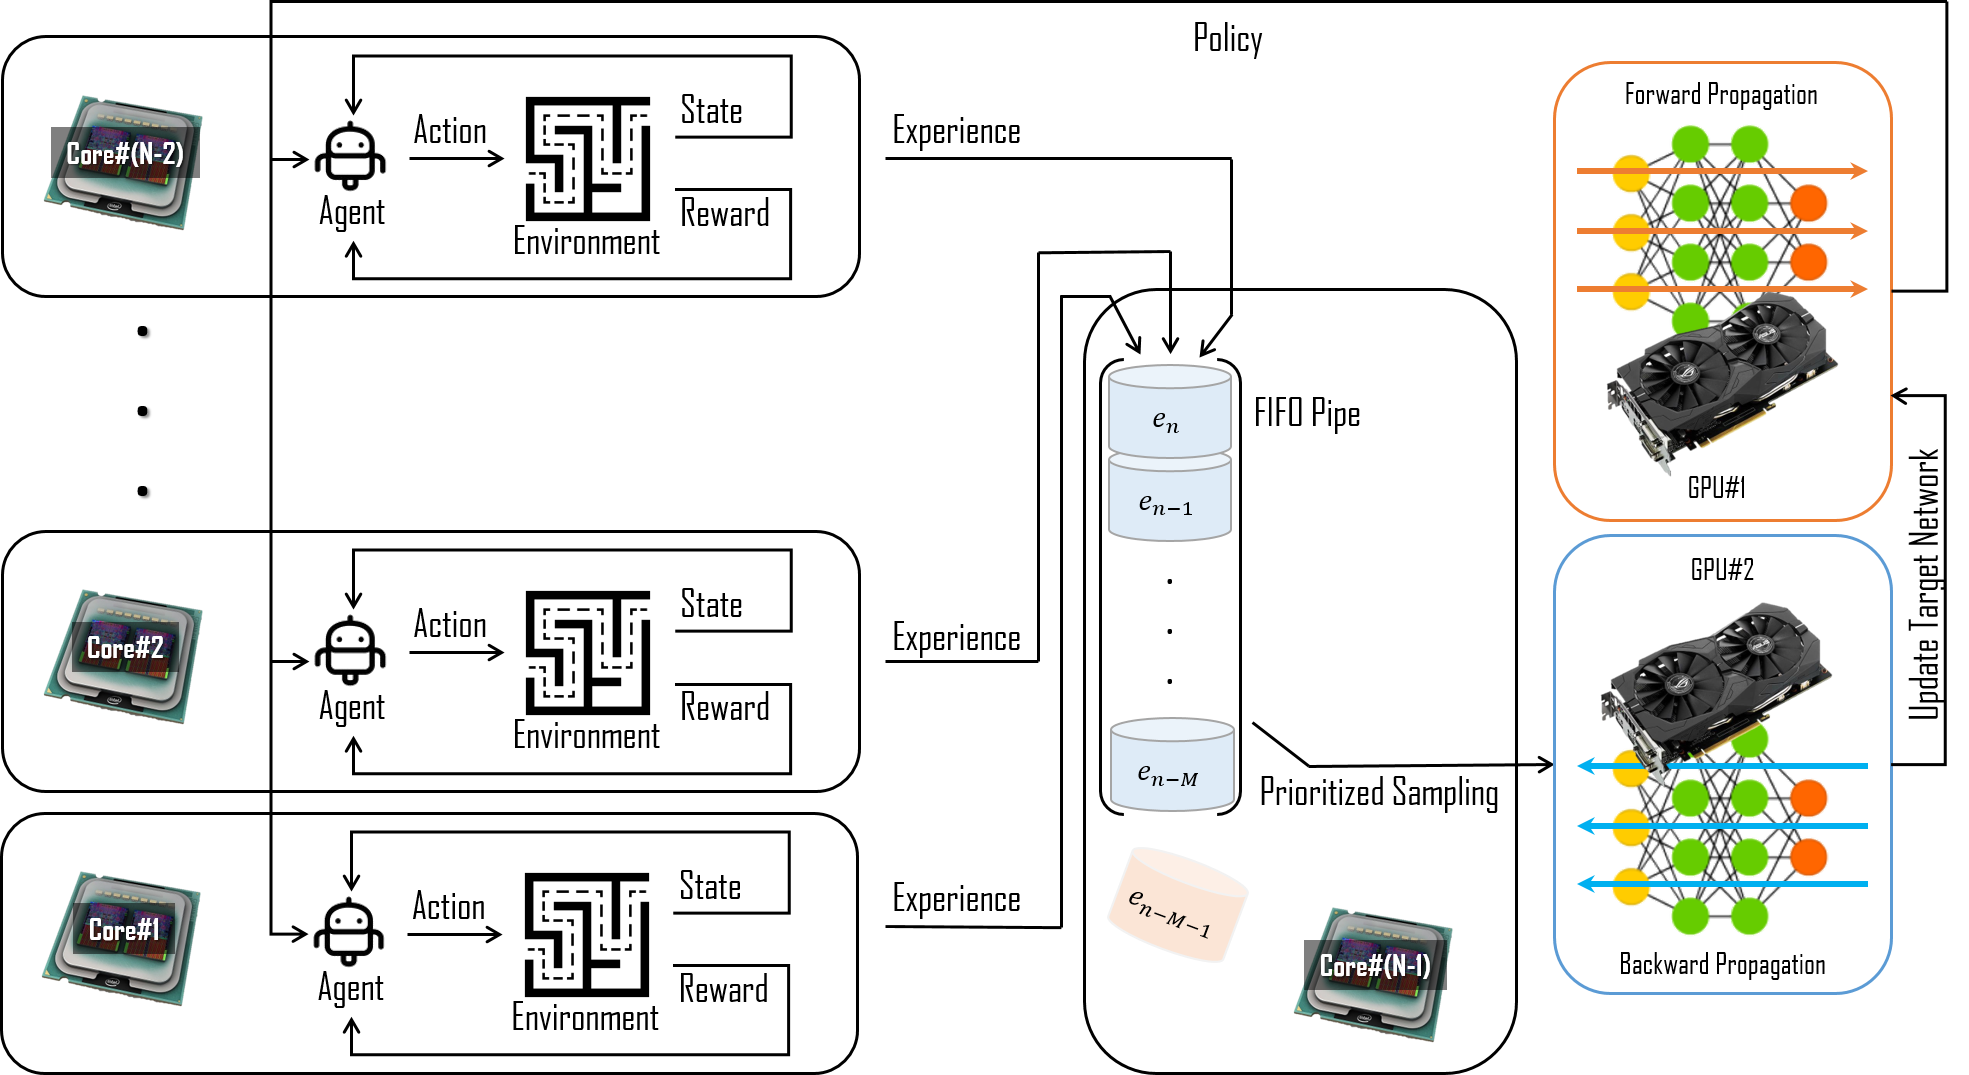
\includegraphics[width=1\textwidth]{asyncronousArchitecture}
	\end{center}
	\caption{Asyncronous Architecture: Hybrid CPU/GPU system is planned to be utilized for multiagent planning.
		\label{fig:asyncronousArchitecture}}
\end{figure}

\section{PUBLICATIONS ABOUT THE THESIS SUBJECT BEING PREPARED AND/OR SUBMITTED}
% Revised
According to time plan, the publications will be prepared prior to start of third phase which is Decentralized Multiagent Planning Phase.

%\newpage
\bibliographystyle{ieeetr}
\bibliography{references}

\end{document}
